\section{Results}
In figure \ref{aha-fig:graphsize} we present the size of the abstract graph in nodes and edges relative to the size of the original graphs which featured an average 4469 nodes and 16420 edges. 
We look at the effect of increasing the amount of soft obstacles (SO) from 0\% (the original test maps with only one traversable terrain) to 50\%.
We also contrast high and low quality abstractions (denoted HQ and LQ) on a range of cluster sizes $\lbrace 10, 15, 20 \rbrace$ (denoted CS10, CS15 and CS20).
\par \indent
Figure \ref{aha-fig:graphsize} shows the average performance of HQ and LQ abstractions with respect to each cluster size. 
\begin{figure}[htbp]
       \caption{\small{\emph{Nodes and edges in abstract graph (HQ vs LQ). }}}
       \begin{center}
                       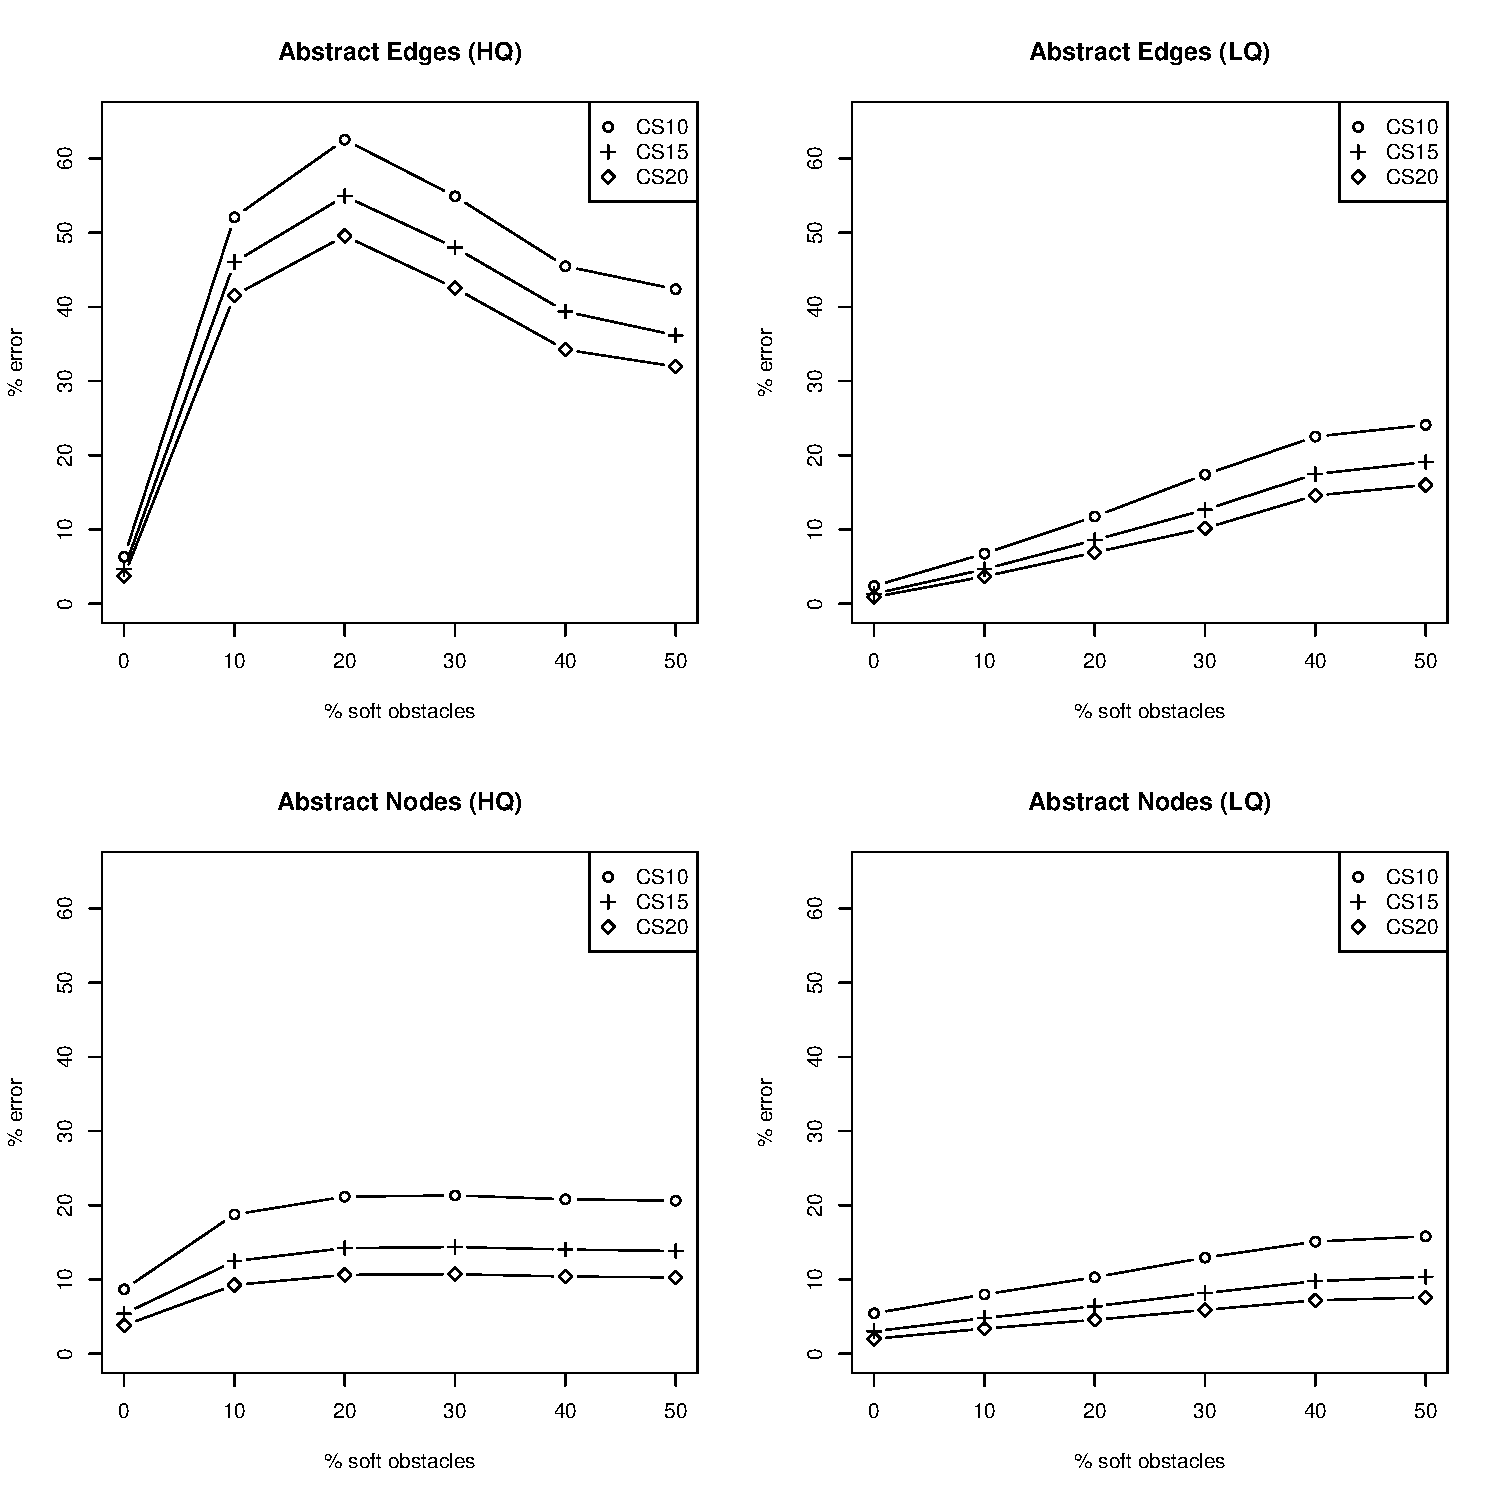
\includegraphics[scale=0.35]{diagrams/graphsize.pdf}
       \end{center}
       \label{aha-fig:graphsize}
\end{figure}
%\input gsntable.tex
The first thing to notice is that on both HQ and LQ abstractions the smallest graphs are generated on the SO 0\% problem set. 
In this case only one traversable terrain exists.
Consequently, most entrances span the length of the border region between adjacent clusters and relatively few transition points are identified. 
From there however we see a very sharp rise in the size of the abstract graph; in the case of HQ abstractions both nodes and edges peak at SO 20\%. 
This observation is consistent with our predictions from lemma \ref{aha-lemma:maxnodes} and lemma \ref{aha-lemma:maxedgesincluster}.
More soft obstacles result in a larger number of smaller entrances for which we require a greater number of nodes and intra-edges to represent.
The increasing number of soft obstacles also results in a much larger number of intra-edges; there are more alternate paths for different sizes and capabilities between each pair of abstract nodes.
Beyond SO 20\% the density of soft obstacles in each cluster makes it harder to find as many paths and consequently less abstract edges are produced. 
Interestingly, the number of nodes remains approximately constant suggesting the number of inter-edges does not increase.
\par \indent
Looking at the LQ graphs, we notice a somewhat different trend. 
Much fewer nodes and edges are generated but both increase linearly up to SO 50\%. 
On maps with few soft obstacles approximately half of all nodes and the majority of edges are dominated. 
As the terrain complexity in each cluster grows however there are less dominated nodes and edges as the circuit condition from theorem \ref{aha-theorem:weakdominance} is less often satisfied.
Consequently, we see see a gradual rise, in both cases peaking at SO 50\%.
\par \indent
As expected, larger clusters result in smaller graphs. 
The difference is largely dependent on the number of soft obstacles in the environment; the largest gap is between CS10 vs. CS20 on SO 50\% using an LQ abstraction.
The CS10 graph in this case was the worst observed LQ abstraction with an node count 15.82\% the size as in the original graph and 24.10\% edges.
If we assume each non-abstract node and edge require one byte of memory to store, then our abstract graph, which contains 2 annotations per edge (capability and clearance, each requiring 1 byte), will still have a space complexity less than 42\% of the original graph even using a naive implementation. 
Custom implementations using bitpacking could eliminate the edge annotation overhead and reduce this further still although the most significant gains appear to come from simply increasing the cluster size; in this case, going from CS10 to CS20 reduces the space complexity to 26.7\%.
\par \indent
Next we consider the performance of AHA* with respect to path quality. We measure this as:
$$ \%error = \frac{apl - opl}{opl} \times 100 $$ where $opl$ is the length of the optimal path as calculated by AA* and $apl$ the length of the abstract path used by AHA*.
Figure \ref{aha-fig:allgraphs}(top) shows the average performance of HQ and LQ abstractions with respect to each cluster size. 
\begin{figure}[htbp]
       \caption{\small{\emph{AHA* performance (HQ vs LQ abstraction). Top: Path quality. Bottom: Search effort. }}}
       \begin{center}
                       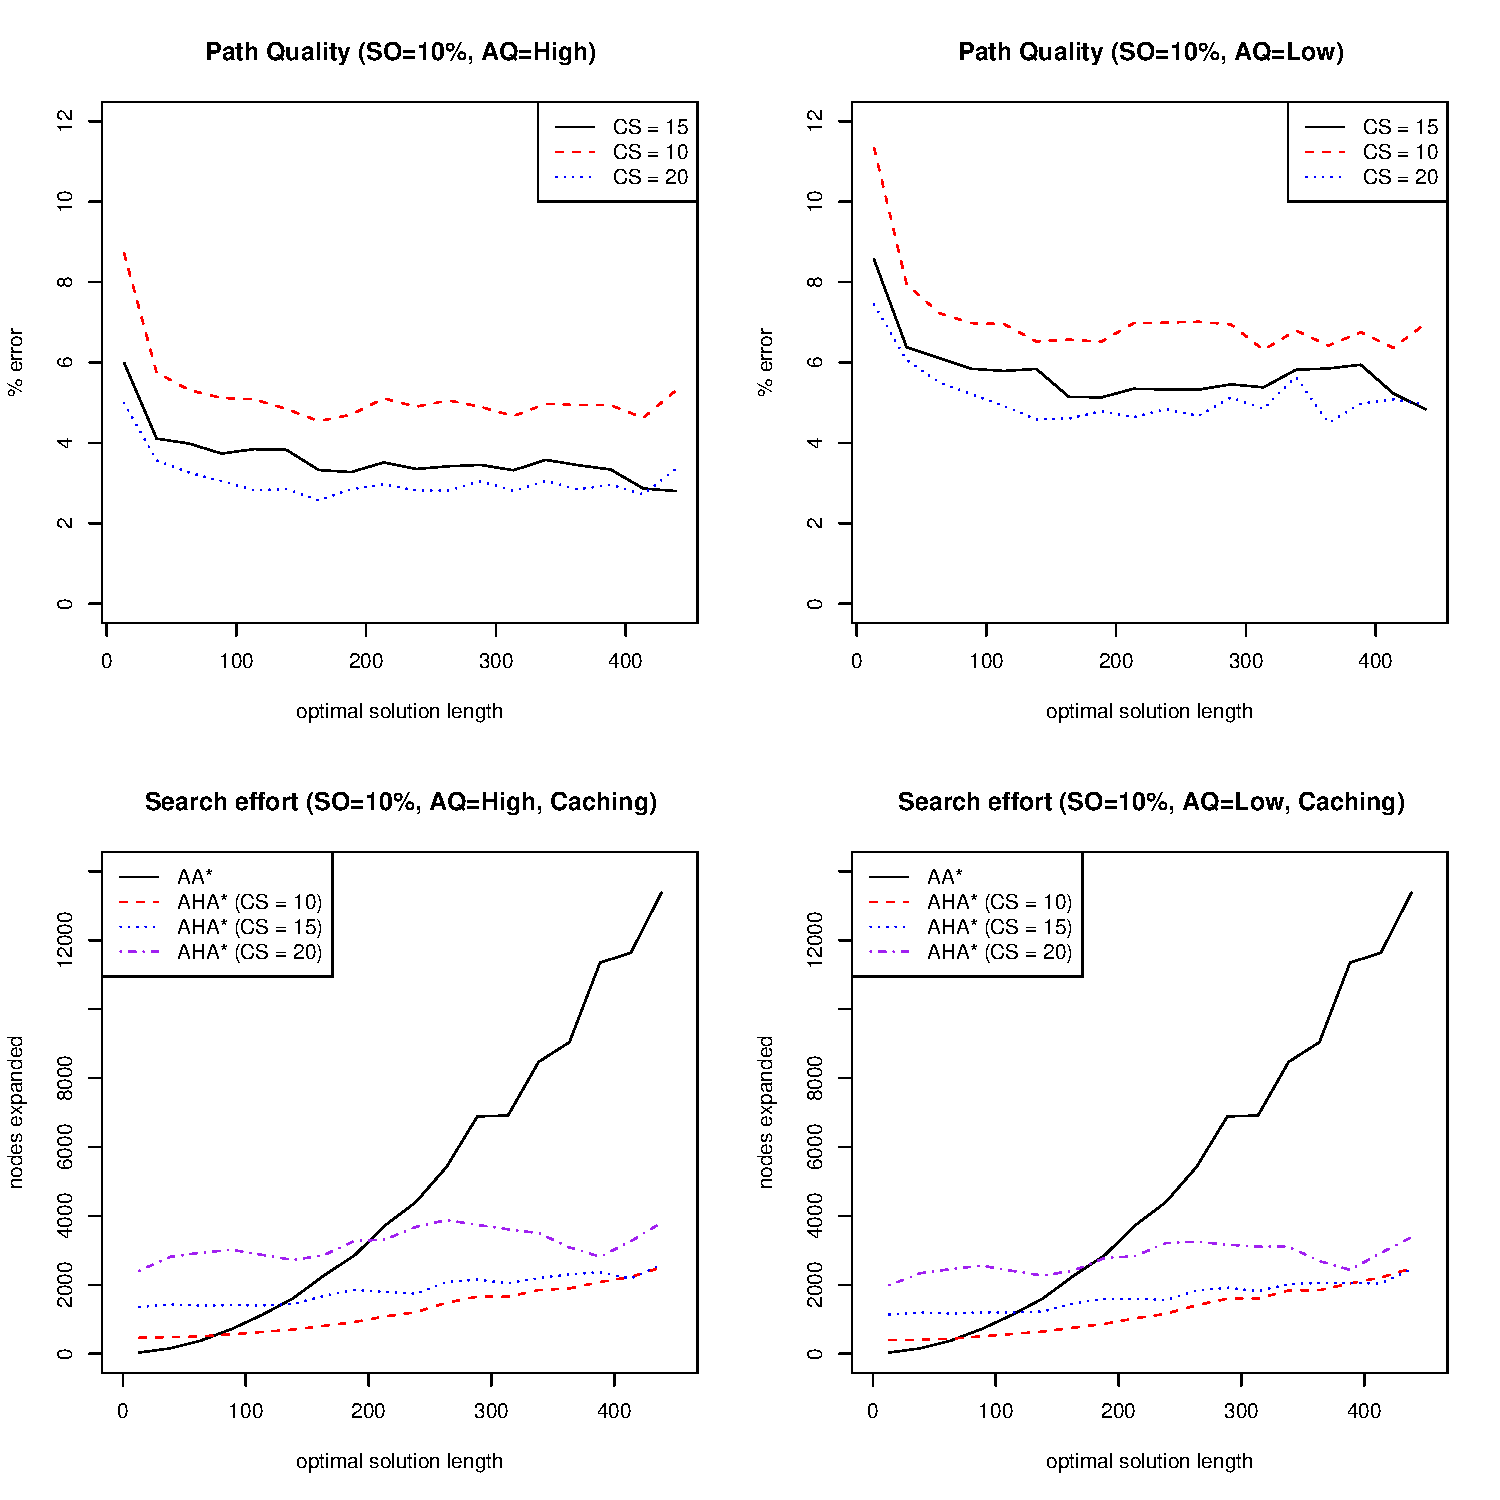
\includegraphics[scale=0.35]{diagrams/allgraphs.pdf}
       \end{center}
       \label{aha-fig:allgraphs}
\end{figure}
Overall, using HQ abstraction yields a very low error for the test, between 2.4 - 4.3\%. 
Perhaps most encouraging however are the results for LQ abstractions, where AHA* performs in the 7-10\% range, giving up relatively little optimality. 
The higher than average error observed for short paths is due to AHA*'s inability to find a direct route from start to goal -- unlike AA*.
As the length of the problem increases this localised error becomes less an issue.
A more complete picture of AHA*'s path quality performance is given in table \ref{aha-table:pathquality} where we observe similar trends. 
\input pqtable.tex
A quick glance confirms initial expectations; bigger clusters result in better performance. 
In some cases however (0\%SO and 5\% SO) going from CS15 LQ to CS20 LQ produces a marginal decrease in quality. 
This seemingly counter-intuitive result can be explained by our inter-edge placement strategy. 
In all situations the pair of nodes with maximal clearance in an entrance tends to be towards the beginning of the entrance which is not an optimal placement. 
On maps that produce low-complexity clusters of predominately one terrain we identify fewer entrances and thus fewer transition points between clusters. 
\cite{botea04} address this issue by placing multiple transition points per entrance whereas we choose only one. 
The biggest increase in path quality is thus observed as we move toward more complex maps which generate more transitions. 
Table \ref{aha-table:pathquality} confirms this; for the SO 10\% set of maps the problem dissapears. 
It appears AHA* is so optimised for complex cases that it suffers some minor performance degredation on simpler problems. 
\par \indent
Finally, we turn our attention to figure \ref{aha-fig:allgraphs}(bottom) where we evaluate AHA* using a search effort metric. 
\input setable.tex
We contrast the total number of nodes expanded by AHA* (insertion + hierarchical search + refinement) with AA*.
A more complete set of results is given in table \ref{aha-table:searcheffort} where we contrast total effort with insertion effort; the latter is presented as a \% of the total.
\par \indent
We observe that the set of HQ experiments using large clusters are disadvantaged in this test. 
The insertion effort required to connect start and goal to each abstract node in their local clusters heavily dominates the total effort causing AHA* CS20 to trail AA* for problems up to length 275.
We can see the gap between CS20 and the smaller cluster sizes decrease as problem size grows but our benchmark set of experiments are not hard enough for such coarse-grain map decompositions to be advantageous. 
The difference is less pronounced using LQ graphs (there are less abstract nodes per cluster) however it appears CS10 or CS15 are more suitable choices for problems up to our maximum length, 450.
